\documentclass[10pt]{scrartcl}

\usepackage[utf8]{inputenc}
\usepackage{tabularx}
\usepackage{longtable}
\usepackage[ngerman]{babel}
\usepackage[automark]{scrpage2}
\usepackage{amsmath,amssymb,amstext}
%\usepackage{mathtools}
\usepackage[]{color}
\usepackage[]{enumerate}
\usepackage{graphicx}
\usepackage{lastpage}
\usepackage[perpage,para,symbol*]{footmisc}
\usepackage{listings} 
\usepackage[pdfborder={0 0 0},colorlinks=false]{hyperref}
\usepackage[numbers,square]{natbib}
\usepackage{color}
\usepackage{colortbl}
\usepackage[absolute]{textpos}
\usepackage{float}
\usepackage[colorinlistoftodos,textsize=small,textwidth=2cm,shadow,bordercolor=black,backgroundcolor={red!100!green!33},linecolor=black]{todonotes}

\lstset{numbers=left, numberstyle=\tiny, numbersep=5pt, breaklines=true, showstringspaces=false} 
\restylefloat{figure}

%changehere
\def\titletext{Praktikum 1 : Stellen/Transitionsnetze}
\def\titletextshort{Praktikum 1}
\author{André Harms, Oliver Steenbuck}

\title{\titletext}

%changehere Datum der Übung
\date{06.06.2012}

\pagestyle{scrheadings}
%changehere
\ihead{TH1, Padberg}
\ifoot{Generiert am:\\ \today}


\cfoot{Oliver Steenbuck, André Harms}


\ohead[]{\titletextshort}
\ofoot[]{{\thepage} / \pageref{LastPage}}

\setlength{\parindent}{0.0in}
\setlength{\parskip}{0.1in}

\begin{document}
\maketitle

\setcounter{tocdepth}{3}
\tableofcontents

%	\listoftables                                 												% 
	\listoffigures  
%	\lstlistoflistings	

\section{Aufgabe 1}
	\subsection{Punkt 1}
				Kein Zusammenhang
				\begin{figure}[H]
    				\centering	
					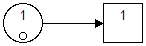
\includegraphics[scale=0.5]{aufg011.png}		
            		\caption{Lebendig, nicht reversibel}
				\end{figure}
				\begin{figure}[H]
    				\centering	
					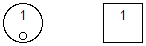
\includegraphics[scale=0.5]{aufg012.png}		
            		\caption{Nicht Lebendig, reversibel}
				\end{figure}
				\begin{figure}[H]
    				\centering	
					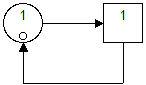
\includegraphics[scale=0.5]{aufg013.png}		
            		\caption{Lebendig, reversibel}
				\end{figure}
				\begin{figure}[H]
    				\centering	
					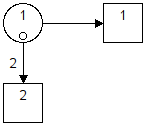
\includegraphics[scale=0.5]{aufg014.png}		
            		\caption{Nicht Lebendig, nicht reversibel}
				\end{figure}
				
	\subsection{Punkt 2}
	Kein Zusammenhang
				\begin{figure}[H]
    				\centering	
					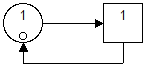
\includegraphics[scale=0.5]{aufg021.png}		
            		\caption{Lebendig, Beschränkt}
				\end{figure}
				\begin{figure}[H]
    				\centering	
					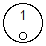
\includegraphics[scale=0.5]{aufg022.png}		
            		\caption{Nicht Lebendig, Beschränkt}
				\end{figure}
				\begin{figure}[H]
    				\centering	
					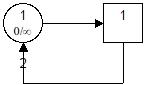
\includegraphics[scale=0.5]{aufg023.png}		
            		\caption{Lebendig, nicht Beschränkt}
				\end{figure}
				\begin{figure}[H]
    				\centering	
					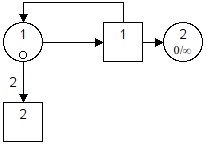
\includegraphics[scale=0.5]{aufg024.png}		
            		\caption{Nicht Lebendig, nicht Beschränkt}
				\end{figure}

		\subsection{Punkt 4}
		Sei Erreichbarkeit definiert als die Erreichbarkeit aller Markierungen in $N$ von $N_{M0}$ also $\forall M \in EG | M \textit{ ist Erreichbar von } N_{M0}$ dann gilt Lebendigeit $\Longrightarrow$ Erreichbarkeit umgekehrt gilt dies nicht da für Erreichbarkeit nur der Hinweg gefordert ist.
		
		
		\subsection{Punkt 7}
		Kein Zusammenhang zwischen positiven Invarianten und Lebendigkeit.
				\begin{figure}[H]
    				\centering	
					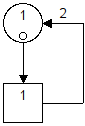
\includegraphics[scale=0.5]{aufg071.png}		
            		\caption{NichtInvariant, Lebendig}
				\end{figure}
				\begin{figure}[H]
    				\centering	
					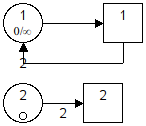
\includegraphics[scale=0.5]{aufg072.png}		
            		\caption{Nicht Invariant, Nicht Lebendig}
				\end{figure}
				\begin{figure}[H]
    				\centering	
					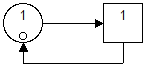
\includegraphics[scale=0.5]{aufg073.png}		
            		\caption{Invariant, Lebendig}
				\end{figure}
				\begin{figure}[H]
    				\centering	
					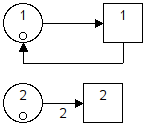
\includegraphics[scale=0.5]{aufg074.png}		
            		\caption{Invariant, Nicht Lebendig}
				\end{figure}
				
		\subsection{Punkt 11}
		Echt positive (alle Elemente positiv) T Invarianten $\Longleftrightarrow$ Lebendigkeit
		
		\subsection{Punkt 16}
		Sei $W_{all}(k)$ ein Weg der alle Knoten eines Graphen beinhaltet und bei $k$ startet und endet.
		So gilt $\forall u \in UG | \exists  W_{all}(u) \Longleftrightarrow \textit{Lebendigkeit}$		
		
		\subsection{Punkt 22}
		$|KG| = 0 \Longleftrightarrow Lebendigkeit$	
		
		\subsection{Punkt 29}
		Verklemmung $\Longrightarrow$ nicht Lebendig und Lebendig $\Longrightarrow$ keine Verklemmung.
		
		\subsection{Punkt 3}
		Kein Zusammenhang zwischen Beschränktheit und Reversibilität.
				\begin{figure}[H]
    				\centering	
					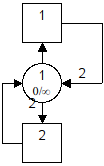
\includegraphics[scale=0.5]{aufg031.png}		
            		\caption{Nicht Beschränkt, Reversibel}
				\end{figure}
				\begin{figure}[H]
    				\centering	
					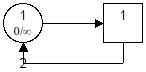
\includegraphics[scale=0.5]{aufg032.png}		
            		\caption{Nicht Beschränkt, Nicht Reversibel}
				\end{figure}
				\begin{figure}[H]
    				\centering	
					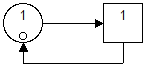
\includegraphics[scale=0.5]{aufg033.png}		
            		\caption{Beschränkt, Reversibel}
				\end{figure}
				\begin{figure}[H]
    				\centering	
					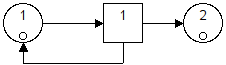
\includegraphics[scale=0.5]{aufg034.png}		
            		\caption{Beschränkt, Nicht Reversibel}
				\end{figure}
		
		
		\subsection{Punkt 5} 
		Reversibilität ist ein Spezialfall von Erreichbarkeit nämlich: $\forall m \in EG | M_0 \textit{ ist erreichbar}$
		
		\subsection{Punkt 8}
		Kein Zusammenhang zwischen P Invarianten und Reversibilität.
				\begin{figure}[H]
    				\centering	
					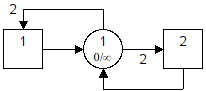
\includegraphics[scale=0.5]{aufg081.png}		
            		\caption{Nicht Invariant, Reversibel}
				\end{figure}
				\begin{figure}[H]
    				\centering	
					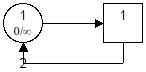
\includegraphics[scale=0.5]{aufg082.png}		
            		\caption{Nicht Invariant, Nicht Reversibel}
				\end{figure}
				\begin{figure}[H]
    				\centering	
					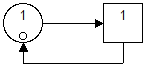
\includegraphics[scale=0.5]{aufg083.png}		
            		\caption{Invariant, Reversibel}
				\end{figure}
				\begin{figure}[H]
    				\centerin g	
					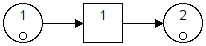
\includegraphics[scale=0.5]{aufg084.png}		
            		\caption{Invariant, Nicht Reversibel}
				\end{figure}
					
\end{document}

